% Chapter 12
\section{Introduction to Recurrent Neural Networks}\label{chap:rnn}
\graphicspath{{assets/lec7/}{assets/lec9/}{assets/lec14/}}

\begin{tcolorbox}[summarybox,title={Learning Outcomes}]
\begin{itemize}
    \item Explain why recurrent structures are needed for sequence modeling and contrast them with feedforward nets.
    \item Derive the forward dynamics and backpropagation-through-time (BPTT) updates for vanilla RNN cells.
    \item Recognize practical stabilization techniques (gradient clipping, gating, normalization) that motivate later LSTM/Transformer chapters.
\end{itemize}
\end{tcolorbox}

\Cref{chap:cnn} showed how architectural bias (convolution/pooling) can replace some data demands while keeping the same optimization loop. This chapter turns to sequences, where the missing ingredient is memory: the model must remember enough of the past to act in the present. The roadmap in \Cref{fig:roadmap} flags this as the sequential branch of the neural strand.

\begin{tcolorbox}[summarybox,title={Design motif}]
Add recurrence, then train it by unrolling time and reusing the backprop machinery from \Cref{chap:backprop}.
\end{tcolorbox}

\subsection{Quick recap: padding in CNNs}

For a 1D or 2D convolution with input size \(n\), kernel size \(k\), stride \(s\), and padding \(p\), the output size is
\[
\left\lfloor \frac{n + 2p - k}{s} \right\rfloor + 1.
\]
When \(s=1\) and you want to preserve the original size, choose \(p=(k-1)/2\) for odd \(k\); padding \(p\) means adding \(p\) zeros on each side (left/right in 1D, all borders in 2D). This bookkeeping matters later when we compare sequence padding to spatial padding in CNNs.

\subsection{Autoencoders and latent representations}

Autoencoders map an input \(\mathbf{x}\) through an \emph{encoder} to a latent vector \(\mathbf{z}\), then reconstruct \(\hat{\mathbf{x}}\) with a \emph{decoder}. Training uses the input itself as the target, so the loss penalizes reconstruction error. An \emph{undercomplete} bottleneck (\(\dim \mathbf{z} < \dim \mathbf{x}\)) behaves like compression; an \emph{overcomplete} latent space can still learn useful structure when paired with regularization. We mention autoencoders here because the idea of encoding a long input into a compact representation will reappear in sequence models.

The statistical learning chapters (\Crefrange{chap:supervised}{chap:logistic}) established the basic training loop: choose a model class, define a loss, optimize it, and then audit generalization and calibration. The feedforward neural chapters then extended the model class from linear predictors to multilayer networks (MLPs, RBF networks, and CNNs). Those architectures have proven effective for tasks such as classification, regression, and feature extraction, but they share a common structural limitation: information flows strictly from input to output, without an internal state that can store context over time.

\subsection{Motivation for Recurrent Neural Networks}

Before delving into the architecture and mathematics of RNNs, it is important to understand why feedforward networks are insufficient for certain applications. Consider the following scenario:

\begin{quote}
\textit{You want to predict an output at time $t$ based not only on the input at time $t$, but also on inputs from previous time steps $t-1, t-2, \ldots, t-k$.}
\end{quote}

This is a common situation in many real-world problems, such as:

\begin{itemize}
    \item Time series forecasting (e.g., stock prices, weather data)
    \item Natural language processing (e.g., predicting the next word in a sentence)
    \item Speech recognition and synthesis
    \item Control systems with memory of past states
\end{itemize}

Order carries meaning even in simple settings: if today is Saturday, the next day is Sunday. In language, ``out of the blue'' means something sudden, whereas ``the ball was blue'' refers to color; the sequence makes the difference. In predictive text, ``I want to buy ...'' favors a different continuation than ``Write a book about Teddy ...'' These examples also highlight variable-length inputs: a review can be three words or three hundred. You can always build a fixed window of past inputs and feed it to a standard MLP, but that approach scales poorly as the history grows and does not share parameters across time.

Feedforward networks treat each input independently and do not have an inherent mechanism to remember or utilize past inputs. To incorporate past information, one might consider explicitly including previous inputs as part of the current input vector, but this approach quickly becomes impractical as the history length grows.

\subsection{Key Idea: State and Memory in RNNs}

Recurrent neural networks address this limitation by introducing a \emph{state vector} $\mathbf{h}_t$ that summarizes information from all previous inputs up to time $t$. The state is updated recursively as new inputs arrive, allowing the network to maintain a form of memory.

Formally, at each time step $t$, the RNN receives an input vector $\mathbf{x}_t$ and updates its hidden state $\mathbf{h}_t$ according to a function $f$ parameterized by weights $\theta$:

\begin{align}
    \mathbf{h}_t = f(\mathbf{h}_{t-1}, \mathbf{x}_t; \theta)
    \label{eq:rnn_state_update}
\end{align}

The output $\mathbf{y}_t$ at time $t$ is then computed as a function of the current state:

\begin{align}
    \mathbf{y}_t = g(\mathbf{h}_t; \theta')
    \label{eq:rnn_output}
\end{align}

Here, $f$ and $g$ are typically nonlinear functions implemented by neural network layers, and $\theta, \theta'$ are learned parameters.

\paragraph{Interpretation:} The hidden state $\mathbf{h}_t$ acts as a \emph{summary} or \emph{encoding} of the entire input history $\{\mathbf{x}_1, \mathbf{x}_2, \ldots, \mathbf{x}_t\}$. This allows the network to make predictions that depend on the temporal context, not just the current input.

\paragraph{Parameter sharing across time.} The same weights are reused at each time step. In the simplest formulation there are three learned matrices: \(W_{xh}\) (input to state), \(W_{hh}\) (state to state), and \(W_{hy}\) (state to output). When you unroll the recurrence, these matrices appear at every step, so the model learns a single transition rule rather than a separate set of parameters for each position in the sequence.

Unrolling makes the training graph \(T\) steps deep. Gradients from each time step accumulate onto the shared weights, and the repeated Jacobian products are precisely why long sequences revive the vanishing/exploding gradient issues from deep feedforward networks.
Training this unrolled graph with standard backpropagation is known as \emph{backpropagation through time} (BPTT).

Recurrent neural networks (RNNs) were among the first practical sequence models \citep{Elman1990,Bengio1994}. CNNs from \Cref{chap:cnn} trade recurrence for parallel, spatially shared filters, while \Cref{chap:transformers} will revisit sequence modeling without recurrence. \Cref{chap:nlp} supplies the embeddings and perplexity metrics commonly paired with RNNs.

\subsection{Comparison with Feedforward Networks}

To contrast, a feedforward network computes the output at time $t$ as:

\begin{align}
    \mathbf{y}_t = \psi(\mathbf{x}_t; \theta)
    \label{eq:ffn_output}
\end{align}

where $\psi$ is a nonlinear function without any dependence on past inputs. This limits the ability of feedforward networks to model temporal dependencies unless the input vector $\mathbf{x}_t$ explicitly contains past information.

\paragraph{Summary:} RNNs extend feedforward networks by incorporating a recurrent connection that allows information to persist across time steps, enabling modeling of sequences and temporal dynamics.

\begin{tcolorbox}[summarybox,title={Shape reminder}]
We keep the row-major (deep-learning) convention: \(\mathbf{x}_t \in \mathbb{R}^{d_x}\), \(\mathbf{h}_t \in \mathbb{R}^{d_h}\), pre-activation \(\mathbf{a}_t = \mathbf{x}_t W_{xh} + \mathbf{h}_{t-1} W_{hh} + \mathbf{b}_h\), output \(\mathbf{y}_t = \mathbf{h}_t W_{hy} + \mathbf{b}_y\). Column-vector formulations simply transpose the order of factors; all stability conclusions (spectral norms of Jacobian factors) carry over.
\end{tcolorbox}

\begin{tcolorbox}[summarybox,title={Simple RNN at a glance}]
\begin{itemize}
    \item \textbf{Objective:} Minimize cross\hyp{}entropy (or another sequence loss) between targets and \(p_\theta(y_t\mid h_t)\), with \(h_t = f(x_t W_{xh} + h_{t-1} W_{hh} + b_h)\).
    \item \textbf{Key hyperparameters:} Hidden state size, BPTT truncation window, optimizer/learning rate, regularization (dropout, weight decay), gradient-clipping threshold.
    \item \textbf{Defaults:} \(\tanh\) or ReLU activations, hidden size 128--512, Adam or SGD+momentum with clipping, layer norm or gating (LSTM/GRU) for long sequences.
    \item \textbf{Common pitfalls:} Vanishing/exploding gradients on long sequences, too-small hidden states, and train/test mismatch when teacher forcing is not reflected at inference.
\end{itemize}
\end{tcolorbox}

\subsection{Outline of this chapter}

In this chapter, we will:

\begin{itemize}
    \item Revisit CNN padding and autoencoders as a bridge to sequence encoders.
    \item Formally define the architecture of recurrent neural networks.
    \item Derive the forward and backward passes for training RNNs.
    \item Discuss challenges such as vanishing and exploding gradients.
    \item Introduce variants of RNNs designed to mitigate these challenges.
    \item Explore applications where RNNs provide significant advantages over feedforward networks.
\end{itemize}

\begin{tcolorbox}[summarybox,title={Vanilla RNN cell (forward + BPTT)}]
\begin{verbatim}
# Forward for a sequence {x_t, y_t}
h_0 = 0
for t = 1..T:
    pre_h = h_{t-1} W_hh + x_t W_xh + b_h
    h_t  = tanh(pre_h)
    yhat_t = h_t W_hy + b_y

# Backward (BPTT with optional truncation K)
delta_pre_next = 0
for t = T..1:
    delta_y = grad_loss(yhat_t, y_t)
    grad_W_hy += h_t^T delta_y
    grad_b_y += delta_y
    delta_h = delta_y W_hy^T + delta_pre_next W_hh^T
    delta_pre = delta_h .* (1 - h_t^2)
    grad_W_hh += h_{t-1}^T delta_pre
    grad_W_xh += x_t^T delta_pre
    grad_b_h += delta_pre
    delta_pre_next = delta_pre
    if t < T-K: break  # truncated BPTT
\end{verbatim}
Use gradient clipping (e.g., clip the global norm of parameter gradients) and layer/batch normalization when sequences are long to avoid exploding/vanishing gradients.
\end{tcolorbox}
The element-wise product in the backward step corresponds to the Hadamard factors described in the derivation in \Cref{chap:mlp}; we write it as \texttt{.*} to align with NumPy/Matlab notation.

\paragraph{Code--math dictionary.} In code blocks we use ASCII identifiers such as \texttt{h\_t}, \texttt{W\_hh}, and \texttt{b\_h}; in equations the same objects appear as \(\mathbf{h}_t\), \(\mathbf{W}_{hh}\), and \(\mathbf{b}_h\) (boldface for vectors/matrices, subscripts for time and role).

Detailed algebraic derivations (forward/backward passes and gradient expressions) appear in \Crefrange{eq:simple_rnn_hidden}{eq:simple_rnn_output}; readers are encouraged to work through the accompanying examples to solidify intuition.

\subsection{Recap: Feedforward Building Blocks}

RNNs reuse the same ingredients as multilayer perceptrons (activations, nonlinear decision boundaries, loss functions, and training heuristics) but wrap them around a temporal axis. \Cref{fig:backprop-computational-graph} from \Cref{chap:backprop} highlights the canonical MLP dataflow along with common activation choices and derivatives that govern gradient flow.

Two-dimensional toy datasets remain useful for reasoning about inductive biases. \Cref{fig:lec7-boundaries} contrasts logistic regression and a shallow MLP on the moons dataset, illustrating how additional hidden units carve nonlinear boundaries that RNN readouts later rely on when decoding the final state.

\begin{figure}[t]
    \centering
    \begin{tikzpicture}
        \begin{groupplot}[
            group style={group size=2 by 1, horizontal sep=1cm},
            width=0.43\linewidth,
            height=0.38\linewidth,
            xmin=-1.2, xmax=1.6,
            ymin=-0.8, ymax=1.4,
            xlabel={$x_1$},
            ylabel={$x_2$},
            axis equal,
            legend style={at={(0.03,0.03)},anchor=south west,legend columns=2,fill=white,draw=none}
        ]
            \nextgroupplot[title={Logistic regression}]
                \addplot+[only marks, mark=*, color=cbBlue, mark size=1.6pt] coordinates {
                    (0.1,0.4) (0.3,0.8) (-0.1,0.9) (-0.4,0.6) (-0.6,0.2)
                    (-0.3,0.1) (-0.7,0.55) (-0.2,0.35) (0.2,1.0) (0.5,0.6)
                };
                \addlegendentry{Class 1}
                \addplot+[only marks, mark=square*, color=cbOrange, mark size=1.6pt] coordinates {
                    (0.4,-0.2) (0.8,-0.3) (1.0,0.1) (0.6,-0.5) (0.2,-0.4)
                    (-0.2,-0.3) (-0.5,-0.4) (0.9,0.35) (1.2,0.2) (0.6,0.2)
                };
                \addlegendentry{Class 2}
                \addplot[thick, color=black] coordinates {(-1.2,-0.2) (1.6,0.6)};
                \node[anchor=west, font=\scriptsize] at (axis cs:0.9,0.65){$w^\top x + b = 0$};
            \nextgroupplot[title={Shallow MLP}]
                \addplot+[only marks, mark=*, color=cbBlue, mark size=1.6pt] coordinates {
                    (0.1,0.4) (0.3,0.8) (-0.1,0.9) (-0.4,0.6) (-0.6,0.2)
                    (-0.3,0.1) (-0.7,0.55) (-0.2,0.35) (0.2,1.0) (0.5,0.6)
                };
                \addplot+[only marks, mark=square*, color=cbOrange, mark size=1.6pt] coordinates {
                    (0.4,-0.2) (0.8,-0.3) (1.0,0.1) (0.6,-0.5) (0.2,-0.4)
                    (-0.2,-0.3) (-0.5,-0.4) (0.9,0.35) (1.2,0.2) (0.6,0.2)
                };
                \addplot[cbGreen, thick, domain=-1.2:1.4, samples=200]
                    {0.35 + 0.55*sin(deg(2.1*x)) - 0.1*x};
                \node[anchor=west, font=\scriptsize, cbGreen] at (axis cs:0.9,0.95){Nonlinear separator};
        \end{groupplot}
    \end{tikzpicture}
    \caption{Schematic: Decision boundaries for logistic regression (left) versus a shallow MLP (right). Linear models carve a single hyperplane, whereas hidden units can warp the boundary to follow non-convex manifolds such as the moons dataset.}
    \label{fig:lec7-boundaries}
\end{figure}

Finally, \Cref{fig:lec7-loss-hyperparams} summarizes two diagnostics: BCE geometry and the effect of learning\hyp{}rate schedules/early stopping.
Here BCE (binary cross\hyp{}entropy) for a binary target $y\in\{0,1\}$ and logit $z$ is $\mathcal{L}(z,y)=\log(1+e^{-z})$ for $y{=}1$ and $\log(1+e^{z})$ for $y{=}0$; the \emph{logit} $z$ is the pre\hyp{}sigmoid score so that $\sigma(z)$ yields the predicted probability. The middle panel contrasts a conservative schedule (smooth decay) with a more aggressive one (faster initial drop but risk of oscillation), and the right panel shows early stopping triggered when validation loss ceases to improve while training loss continues decreasing.
We will reuse these when tuning sequence models, where overfitting appears as a divergence between per\hyp{}token training and validation likelihood.

\begin{tcolorbox}[summarybox,title={Author's note: treat early stopping as the default brake}]
Unless there is a compelling reason to run to numerical convergence, stop as soon as the validation curve flattens while the training curve keeps dropping. Checkpoint the best weights and resume only if new data or regularization changes warrant it. That simple rule prevents most runaway experiments without elaborate hyperparameter sweeps.
\end{tcolorbox}

\begin{figure}[t]
    \centering
    \begin{tikzpicture}
        \begin{groupplot}[
            group style={group size=3 by 1, horizontal sep=1.2cm},
            width=0.32\linewidth, height=0.36\linewidth
        ]
        % BCE vs logit
        \nextgroupplot[
            title={BCE vs logit $z$},
            xlabel={$z$},
            ylabel={$\mathcal{L}$},
            xmin=-6, xmax=6,
            ymin=0, ymax=6,
            legend style={at={(0.97,0.97)},anchor=north east,fill=white,draw=none}
        ]
            \addplot[cbBlue, thick, samples=200, domain=-6:6] {ln(1+exp(-x))}; \addlegendentry{$y{=}1$}
            \addplot[cbOrange, dashed, thick, samples=200, domain=-6:6] {ln(1+exp(x))}; \addlegendentry{$y{=}0$}
        % Learning-rate effect (schematic loss curves)
        \nextgroupplot[
            title={Learning rate effect},
            xlabel={epoch},
            ylabel={loss},
            xmin=0, xmax=50,
            ymin=0, ymax=1.2,
            legend style={at={(0.97,0.97)},anchor=north east,fill=white,draw=none}
        ]
            \addplot[cbBlue, thick, samples=100, domain=0:50] {0.2 + 0.9*exp(-x/12)}; \addlegendentry{conservative}
            \addplot[cbPink, dashed, thick, samples=100, domain=0:50] {0.15 + 1.0*exp(-x/6) + 0.05*sin(0.6*x)}; \addlegendentry{aggressive}
        % Early stopping (train vs val)
        \nextgroupplot[
            title={Early stopping},
            xlabel={epoch},
            ylabel={loss},
            xmin=0, xmax=50,
            ymin=0, ymax=1.2,
            legend style={at={(0.97,0.97)},anchor=north east,fill=white,draw=none}
        ]
            \addplot[cbGreen, thick, samples=100, domain=0:50] {0.1 + 0.9*exp(-x/10)}; \addlegendentry{train}
            % U-shaped validation curve: improves early, then degrades (overfitting).
            \addplot[cbOrange, dashed, thick, samples=200, domain=0:50] {0.25 + 0.7*exp(-x/12) + 0.0004*(x-20)^2}; \addlegendentry{val}
            \addplot[gray!70, dashed] coordinates {(20,0) (20,1.2)};
            \node[font=\scriptsize, anchor=south west, gray!70] at (axis cs:20,0.08) {stop};
        \end{groupplot}
    \end{tikzpicture}
    \ifdefined\HCode
        \caption{Schematic: Binary cross-entropy geometry (left), effect of learning-rate schedules on loss (middle), and the typical training/validation divergence that motivates early stopping (right).}
    \else
        % Avoid inline math in captions; it wraps poorly in some EPUB renderers.
        \caption{Schematic: Binary cross-entropy geometry (left), effect of learning-rate schedules on loss (middle), and the typical training/validation divergence that motivates early stopping (right).}
    \fi
    \label{fig:lec7-loss-hyperparams}
\end{figure}

\begin{tcolorbox}[summarybox,title={LayerNorm and residual RNN tips}]
Layer Normalization~\citep{Ba2016} stabilizes recurrent dynamics by normalizing each hidden vector \(h_t\) across features before applying the nonlinearity; unlike BatchNorm it works with batch size 1 and handles variable-length sequences gracefully. Residual RNN stacks (adding the input of a layer back to its output) keep gradients flowing even when depth increases, mirroring the skip-connections that make deep CNNs trainable. Together, LayerNorm + residual links curb exploding/vanishing gradients and are the default when building multi-layer RNN/LSTM stacks.
\end{tcolorbox}

\paragraph{Historical Note: Hopfield Networks}

An early influential recurrent network is the Hopfield network \citep{Hopfield1982}, which is a form of associative memory. Unlike modern RNNs, Hopfield networks have symmetric weights and are designed to converge to stable states representing stored patterns. While Hopfield networks are not directly used for sequence modeling, they helped establish the energy-based viewpoint that reappears in later recurrent and attention-based models.

Bidirectional extensions run two RNNs in opposite directions and concatenate their states; they are widely used in encoders for labeling tasks when the full context is available.

\subsection{Input--output configurations and mathematical formulation}

RNNs can map sequences to sequences in several ways:
\begin{itemize}
    \item Many-to-one (e.g., sentiment classification): consume \(x_{1:T}\), emit one label after the final state.
    \item One-to-many (e.g., conditional generation): condition on a context vector, then autoregressively emit a sequence.
    \item Many-to-many (e.g., tagging, ASR): emit \(y_t\) at every step; encoder--decoder variants compress \(x_{1:T}\) then decode.
    \item Bidirectional encoders: run a forward and backward RNN and concatenate the states for sequence labeling or as encoder context.
    \end{itemize}

Consider an input sequence \(\{x_1, x_2, \ldots, x_T\}\), where each \(x_t \in \mathbb{R}^d\). The RNN computes hidden states \(\{h_1, h_2, \ldots, h_T\}\) and outputs \(\{y_1, y_2, \ldots, y_T\}\) as follows:
\begin{align}
h_0 &= \mathbf{0} \quad \text{(initial hidden state)} \\
h_t &= f(x_t W_{xh} + h_{t-1} W_{hh} + b_h), \quad t=1,\ldots,T \label{eq:rnn_hidden_state}\\
y_t &= g(h_t W_{hy} + b_y), \quad t=1,\ldots,T \label{eq:rnn_output_state}
\end{align}

\begin{tcolorbox}[summarybox,title={Shapes and masks (batch $B$, time $T$)}]
Inputs \(X \in \mathbb{R}^{B\times T \times d_x}\); hidden states \(H \in \mathbb{R}^{B\times T \times d_h}\); logits \(Y \in \mathbb{R}^{B\times T \times d_o}\). Parameters (row-major): \(W_{xh}\in\mathbb{R}^{d_x\times d_h}\), \(W_{hh}\in\mathbb{R}^{d_h\times d_h}\), \(W_{hy}\in\mathbb{R}^{d_h\times d_o}\), biases \(b_h\in\mathbb{R}^{d_h}\), \(b_y\in\mathbb{R}^{d_o}\).\\
Padding mask \(M\in\{0,1\}^{B\times T}\): loss \(L=\sum_{b,t} M_{b,t}\,\text{CE}(\hat y_{b,t}, y_{b,t})/\sum_{b,t} M_{b,t}\). Masks preview the padding/causal masks detailed in \Cref{chap:transformers}.
\end{tcolorbox}
\subsection{Recurrent Neural Networks: Historical Context and Motivation}

Recall from our earlier discussion on Hopfield networks that the configuration of the network states significantly impacts the overall energy landscape. The sequence of states, or more precisely, their spatial arrangement within the network, determines the energy and thus the network's behavior. This property endowed Hopfield networks with associative memory capabilities, as the weights were constructed to "remember" specific patterns.

However, Hopfield networks were primarily designed for storage and retrieval of static patterns rather than for dynamic prediction or forecasting tasks. Despite their introduction in 1982, their practical utility beyond research was limited.

\subsection{The 1986 Breakthrough: Backpropagation and Trainable Multi-Layer Networks}

In 1986, Rumelhart, Hinton, and Williams popularized the use of backpropagation as a practical training method for multilayer networks \citep{Rumelhart1986}. That contribution is not an RNN architecture; it is a training procedure that made it feasible to fit large parametric models by propagating error derivatives through compositions of linear maps and nonlinearities.

For recurrent networks, the conceptual move is to view the computation graph as a \emph{shared} module repeated across time steps. Training then becomes standard backpropagation applied to the unrolled graph, with gradients accumulated across each copy of the shared parameters; this is precisely what ``backpropagation through time'' (BPTT) implements in the sections that follow.

\subsection{State Dynamics in Recurrent Neural Networks}

The 1986 RNN formulation introduced the concept of a \emph{state} that evolves over time as a function of the previous state and the current input. Formally, the state update can be expressed as:
\begin{equation}
    \mathbf{h}_t = f(\mathbf{h}_{t-1}, \mathbf{x}_t; \theta).
\end{equation}
where
\begin{itemize}
    \item \(\mathbf{h}_t\) is the hidden state at time \(t\),
    \item \(\mathbf{x}_t\) is the input at time \(t\),
    \item \(f\) is a nonlinear function parameterized by \(\theta\) (e.g., weights and biases),
    \item \(\mathbf{h}_{t-1}\) is the hidden state at the previous time step.
\end{itemize}

The output at time \(t\), denoted \(\mathbf{y}_t\), is typically computed as a function of the hidden state:
\begin{equation}
    \mathbf{y}_t = g(\mathbf{h}_t; \phi).
\end{equation}
where \(g\) is another nonlinear function parameterized by \(\phi\).

\paragraph{Interpretation}

- The hidden state \(\mathbf{h}_t\) acts as a memory that summarizes information from all previous inputs up to time \(t\).
- The recurrence allows the network to maintain context and model temporal dependencies.

\subsection{Unfolding the Recurrent Neural Network}

To better understand and implement RNNs, it is common to \emph{unfold} the network through time. Unfolding transforms the recurrent structure into a feedforward network with shared weights across time steps.

\paragraph{Process}

- Start with an initial hidden state \(\mathbf{h}_0\), which may be initialized to zero or learned.
- At each time step \(t\), compute \(\mathbf{h}_t\) using \Cref{eq:rnn_state_update}.
- Compute output \(\mathbf{y}_t\) using \Cref{eq:rnn_output}.
- The parameters \(\theta\) and \(\phi\) are shared across all time steps, enabling the network to generalize across sequences of varying lengths.

\paragraph{Significance}

- Unfolding clarifies the flow of information and dependencies across time.
- It facilitates the application of backpropagation through time (BPTT) for training.

\subsection{Mathematical Formulation of a Simple RNN Cell}

Consider a simple RNN cell with the following update equations:
\begin{align}
    \mathbf{h}_t &= \sigma_h \left( \mathbf{x}_t \mathbf{W}_{xh} + \mathbf{h}_{t-1} \mathbf{W}_{hh} + \mathbf{b}_h \right), \label{eq:simple_rnn_hidden} \\
    \mathbf{y}_t &= \sigma_y \left( \mathbf{h}_t \mathbf{W}_{hy} + \mathbf{b}_y \right). \label{eq:simple_rnn_output}
\end{align}
\begin{figure}[t]
    \centering
    \begin{tikzpicture}[
        font=\small\sffamily,
        >=Latex,
        node distance=2.4cm,
        box/.style={draw, rounded corners, minimum width=1.8cm, minimum height=0.9cm},
        arrow/.style={->, thick}
    ]
        % Nodes
        \node[box] (h1) at (0,0) {$h_{t-1}$};
        \node[box, right=of h1] (h2) {$h_{t}$};
        \node[box, right=of h2] (h3) {$h_{t+1}$};
        \node (x1) at (0,-1.2) {$x_{t-1}$};
        \node (x2) at (h2|-x1) {$x_{t}$};
        \node (x3) at (h3|-x1) {$x_{t+1}$};
        \node (y1) at (0,1.2) {$y_{t-1}$};
        \node (y2) at (h2|-y1) {$y_{t}$};
        \node (y3) at (h3|-y1) {$y_{t+1}$};
        % Arrows
        \draw[arrow] (h1) -- node[above, font=\scriptsize] {$\mathbf{W}_{hh}$} (h2);
        \draw[arrow] (h2) -- (h3);
        \draw[arrow] (x1) -- node[midway, right, font=\scriptsize, xshift=1mm] {$\mathbf{W}_{xh}$} (h1);
        \draw[arrow] (x2) -- node[midway, right, font=\scriptsize, xshift=1mm] {$\mathbf{W}_{xh}$} (h2);
        \draw[arrow] (x3) -- node[midway, right, font=\scriptsize, xshift=1mm] {$\mathbf{W}_{xh}$} (h3);
        \draw[arrow] (h1) -- node[midway, right, font=\scriptsize, xshift=1mm] {$\mathbf{W}_{hy}$} (y1);
        \draw[arrow] (h2) -- node[midway, right, font=\scriptsize, xshift=1mm] {$\mathbf{W}_{hy}$} (y2);
        \draw[arrow] (h3) -- node[midway, right, font=\scriptsize, xshift=1mm] {$\mathbf{W}_{hy}$} (y3);

        % Shared-parameter annotation: brace anchored to the left/right cells so it
        % stays aligned if the figure spacing changes.
        \coordinate (braceL) at ($(h1.south west)+(0,-12mm)$);
        \coordinate (braceR) at ($(h3.south east)+(0,-12mm)$);
        \draw[decorate, decoration={brace, amplitude=5pt}] (braceL) -- node[midway, below=10pt]{\scriptsize shared parameters across the unrolled sequence} (braceR);
    \end{tikzpicture}
    \caption{Schematic: Unrolling an RNN reveals repeated application of the same parameters across time steps. This view motivates backpropagation through time (BPTT), which accumulates gradients through every copy before updating the shared weights.}
    \label{fig:lec7-rnn-unrolled}
\end{figure}
\subsection{Recurrent Neural Network (RNN) Unfolding and Parameter Sharing}

Recall that a recurrent neural network (RNN) processes sequential data by maintaining a hidden state that evolves over time. At each time step \( t \), the network receives an input \( \mathbf{x}_t \) and updates its hidden state \( \mathbf{h}_t \), which in turn produces an output \( \mathbf{y}_t \). \Cref{fig:lec7-rnn-unrolled} depicts this unfolding explicitly so we can reason about the repeated weight matrices across time.

\paragraph{Unfolding the RNN}
Unfolding the RNN across time steps transforms the recurrent structure into a deep feedforward network with shared weights across layers (time steps). This unrolled network looks like a chain where each hidden state depends on the previous hidden state and the current input:

\[
\mathbf{h}_t = f(\mathbf{h}_{t-1}, \mathbf{x}_t; \Theta), \quad \mathbf{y}_t = g(\mathbf{h}_t; \Theta_y)
\]

where \( f \) and \( g \) are nonlinear functions parameterized by weights \(\Theta\) and \(\Theta_y\), respectively.

\paragraph{Parameter Sharing}
A key property of RNNs is \emph{parameter sharing} across time steps. Specifically:

\begin{itemize}
    \item The weights connecting the previous hidden state \(\mathbf{h}_{t-1}\) to the current hidden state \(\mathbf{h}_t\) are the same for all \( t \).
    \item The weights connecting the input \(\mathbf{x}_t\) to the hidden state \(\mathbf{h}_t\) are also shared across all time steps.
    \item The weights mapping the hidden state \(\mathbf{h}_t\) to the output \(\mathbf{y}_t\) are shared as well.
\end{itemize}

This parameter sharing reduces the number of parameters to learn and enables the network to generalize across different positions in the sequence.

\subsection{Mathematical Formulation of the RNN}

We formalize the RNN update equations as follows. Let the hidden state at time \( t \) be \(\mathbf{h}_t \in \mathbb{R}^{1\times h}\), the input at time \( t \) be \(\mathbf{x}_t \in \mathbb{R}^{1\times d}\), and the output at time \( t \) be \(\mathbf{y}_t \in \mathbb{R}^{1\times o}\) (row-vector convention). Let \(\mathbf{a}_t\in\mathbb{R}^{1\times h}\) denote the pre-activation (affine) hidden update.

\begin{align}
    \mathbf{a}_t &= \mathbf{h}_{t-1}\mathbf{W}_a + \mathbf{x}_t\mathbf{W}_x + \mathbf{b}_h, \\
    \mathbf{h}_t &= f\!\left(\mathbf{a}_t\right), \\
    \mathbf{y}_t &= g\left( \mathbf{h}_t\mathbf{W}_y + \mathbf{b}_y \right),
\end{align}

where:
\begin{itemize}
    \item \(\mathbf{W}_a \in \mathbb{R}^{h \times h}\) is the recurrent weight matrix (hidden-to-hidden).
    \item \(\mathbf{W}_x \in \mathbb{R}^{d \times h}\) is the input-to-hidden weight matrix.
    \item \(\mathbf{W}_y \in \mathbb{R}^{h \times o}\) is the hidden-to-output weight matrix.
    \item \(\mathbf{b}_h \in \mathbb{R}^h\) and \(\mathbf{b}_y \in \mathbb{R}^o\) are bias vectors.
    \item \(f(\cdot)\) is the activation function for the hidden state (commonly \(\tanh\) or \(\mathrm{ReLU}\)).
    \item \(g(\cdot)\) is the output activation function (e.g., softmax for classification).
\end{itemize}
Checking dimensions: \(\mathbf{h}_{t-1}\mathbf{W}_a\in\mathbb{R}^{1\times h}\), \(\mathbf{x}_t\mathbf{W}_x\in\mathbb{R}^{1\times h}\), and \(\mathbf{h}_t\mathbf{W}_y\in\mathbb{R}^{1\times o}\), so the shapes are consistent with the compact form \eqref{eq:rnn_compact}.

\paragraph{Interpretation}
\Cref{eq:rnn_hidden_state} shows that the current hidden state \(\mathbf{h}_t\) is a nonlinear transformation of the previous hidden state \(\mathbf{h}_{t-1}\) and the current input \(\mathbf{x}_t\). \Cref{eq:rnn_output} maps the hidden state to the output at time \( t \).

\paragraph{Reusability of the Hidden State}
The hidden state \(\mathbf{h}_t\) serves as a summary of all previous inputs up to time \( t \). This recursive formulation allows the network to capture temporal dependencies of arbitrary length.

\subsection{Generalized Notation}

To simplify notation, define the concatenated input vector at time \( t \):

\[
\mathbf{z}_t = \begin{bmatrix} \mathbf{h}_{t-1} & \mathbf{x}_t \end{bmatrix} \in \mathbb{R}^{1\times (h + d)}.
\]

Correspondingly, define the combined weight matrix:

\[
\mathbf{W} = \begin{bmatrix} \mathbf{W}_a \\ \mathbf{W}_x \end{bmatrix} \in \mathbb{R}^{(h + d)\times h}.
\]

Then the hidden state update can be written compactly as:

\begin{equation}
    \mathbf{h}_t = \sigma\left( \mathbf{z}_t \mathbf{W} + \mathbf{b}_h \right). \label{eq:rnn_compact}
\end{equation}
This stacks the recurrent and input weights into a single matrix.
\subsection{Recurrent Neural Network (RNN) Architectures and Loss Computation}

Recall from previous discussions that the loss function for classification tasks often involves cross\hyp{}entropy terms of the form:
\begin{equation}
\mathcal{L} = - \sum_{i} y_i \log \hat{y}_i,
\end{equation}
where \( y_i \) is the true label (often one-hot encoded) and \( \hat{y}_i \) is the predicted probability for class \( i \). When \( \hat{y} = y \), the loss is zero, indicating perfect prediction.

In the context of RNNs, the total loss over a sequence is typically the sum of losses at each time step:
\begin{equation}
\mathcal{L}_{\text{total}} = \sum_{t=1}^T \mathcal{L}_t,
\end{equation}
where \( T \) is the sequence length.

\paragraph{Forward and Backward Passes in RNNs}

The forward pass involves propagating inputs through the network over time steps \( t = 1, \ldots, T \), producing outputs \( \hat{y}_t \) at each step. After computing the loss, the backward pass computes gradients with respect to parameters by backpropagating errors through time, a process known as \emph{Backpropagation Through Time} (BPTT).

BPTT unfolds the RNN across time steps and applies standard backpropagation through this unrolled network. The key insight is that parameters are shared across time steps, so gradients accumulate contributions from all time steps; \cref{fig:lec7-bptt} highlights the simultaneous forward flow (black) and backward gradients (pink) that piggyback across every copy.

\begin{tcolorbox}[summarybox,title={Truncated BPTT in practice}]
Unroll \(K\) steps, accumulate loss, backprop through those \(K\) steps, then detach the hidden state to stop graph growth:
\begin{verbatim}
h = h0
for t in range(T):
    h, yhat = rnn(x[t], h)
    loss += mask[t] * CE(yhat, y[t])
    if (t+1) % K == 0:
        loss.backward()
        clip_grad_norm_(model.parameters(), tau)
        opt.step(); opt.zero_grad()
        h = h.detach()  # carry state, drop graph
\end{verbatim}
Choose \(K\) to balance memory and credit assignment (common range: 20--100 steps).
\end{tcolorbox}

\begin{figure}[t]
    \centering
    \begin{tikzpicture}[
        font=\small\sffamily,
        >=Latex,
        arrow/.style={->, thick}
    ]
        % forward chain
        \foreach \i in {0,...,4} {
            \node[draw, rounded corners, minimum width=1.2cm, minimum height=0.7cm] (h\i) at (2*\i,0) {$h_{t+\i}$};
            \node (x\i) at (2*\i,-1.0) {$x_{t+\i}$};
            \draw[arrow] (x\i) -- (h\i);
        }
        \foreach \i/\j in {0/1,1/2,2/3,3/4} {\draw[arrow] (h\i) -- (h\j);}
        % backward (gradient) arrows
        \foreach \i/\k in {1/0,2/1,3/2,4/3} {
            \draw[cbPink, <-, thick] (h\i.north) .. controls +(0,1.0) and +(0,1.0) .. node[above,pos=0.5]{\scriptsize $\partial\mathcal{L}/\partial h_{t+\i}$} (h\k.north);
        }
        % shared parameters note
        \node at (4,-2.0) {\scriptsize shared $(\mathbf{W}_{hh}, \mathbf{W}_{xh}, \mathbf{W}_{hy})$ across time};
    \end{tikzpicture}
    \caption{Schematic: Backpropagation through time (BPTT): unrolled forward pass (black) and backward gradients (pink) through time.}
    \label{fig:lec7-bptt}
\end{figure}

\paragraph{Vanishing and Exploding Gradients}

Because each gradient term contains products of Jacobians such as
\[
\frac{\partial \mathbf{h}_t}{\partial \mathbf{h}_{t-1}} = \mathrm{diag}\!\big( f'(\mathbf{a}_t) \big)\,\mathbf{W}_{hh}^{\top},
\]
with pre\hyp{}activation \(\mathbf{a}_t=\mathbf{x}_t\mathbf{W}_{xh}+\mathbf{h}_{t-1}\mathbf{W}_{hh}+\mathbf{b}_h\) and elementwise nonlinearity \(f\), long sequences multiply many such factors. Here \(\mathbf{W}_{hh}\in\mathbb{R}^{d_h\times d_h}\) and \(\mathrm{diag}\big(f'(\mathbf{a}_t)\big)\in\mathbb{R}^{d_h\times d_h}\), so the Jacobian \(\partial \mathbf{h}_t/\partial \mathbf{h}_{t-1}\) is a \(d_h\times d_h\) matrix. If the spectral norm of each factor is below one the product decays exponentially (vanishing); norms above one cause growth (exploding). \Cref{fig:lec7-vanishing} illustrates both behaviors across time. Practical remedies include gradient clipping, orthogonal or unitary recurrent matrices, layer normalization, and gated architectures (LSTM/GRU) that introduce additive memory paths.
Empirically, vanilla RNNs often fail to preserve dependencies beyond roughly 5--10 steps in language tasks, which is why gated cells became the default for longer sequences.
\begin{figure}[t]
    \centering
    \includegraphics[width=0.72\linewidth]{lec7_vanish_explode}
    \caption{Schematic: Vanishing (blue) versus exploding (orange) gradients on a log scale. The gray strip highlights the stability band; the inset reminds readers that repeated Jacobian products either shrink gradients (thin blue arrows) or amplify them (thick orange arrows).}
    \label{fig:lec7-vanishing}
\end{figure}

\paragraph{Parameter Updates}

At each time step, the gradient of the loss with respect to parameters (e.g., weights \( W \)) depends on the chain of partial derivatives through the network states:
\begin{equation}
\frac{\partial \mathcal{L}}{\partial W} = \sum_{t=1}^T \frac{\partial \mathcal{L}_t}{\partial W}.
\end{equation}
Because of parameter sharing, the same \( W \) influences multiple time steps, and the total gradient is the sum over these contributions.

\subsection{Stabilizing Recurrent Training}

\paragraph{Gradient clipping.} A practical safeguard is to clip the global norm of the gradient when it exceeds a threshold. \Cref{fig:lec7-clipping} shows how clipping prevents the exploding case from destabilizing optimization while leaving the vanishing regime untouched. Orthogonal or unitary initializations for the recurrent weight matrix \(W_{hh}\) are another common trick: because orthogonal matrices preserve Euclidean norms, gradients neither explode nor vanish in the very early stages of training (before nonlinearities and data\hyp{}dependent effects accumulate).

\begin{tcolorbox}[summarybox,title={Rule of thumb: keep gradients in the safe band}]
Spectral norm \(\|\mathbf{W}_{hh}\|_2 \approx 1\) keeps gradients roughly stable over tens of steps; clipping thresholds \(\tau \in [0.5, 5]\) are sensible defaults when sequences are long. BatchNorm inside the recurrent loop is rarely helpful; prefer LayerNorm or gating to stabilize dynamics.
\end{tcolorbox}

\begin{tcolorbox}[summarybox,title={Author's note: do not fight vanilla RNNs}]
If your task needs dependencies longer than a handful of steps, do not over-tune a plain RNN. Start with clipping and a sensible truncation window, but move to GRU/LSTM once you see long-range information vanish.
\end{tcolorbox}

\paragraph{Dropout in RNNs.} Variational/recurrent dropout applies the same dropout mask at every time step to avoid injecting temporal noise \citep{Gal2016,Semeniuta2016}; zoneout preserves hidden units stochastically instead of zeroing them \citep{Krueger2016}. Standard per-time-step dropout often harms sequence retention.

\begin{figure}[t]
    \centering
    \begin{tikzpicture}
        \begin{groupplot}[
            group style={group size=2 by 1, horizontal sep=1.6cm},
            width=0.44\linewidth,
            height=0.35\linewidth,
            xmin=0,xmax=80,
            xlabel={Iteration},
            grid=both,
            minor tick num=1,
            xlabel style={yshift=4pt}
        ]
            \nextgroupplot[
                ylabel={$\|\mathbf{g}\|$},
                ymin=0,ymax=20,
                legend style={at={(0.02,0.95)},anchor=north west},
                ytick={0,5,10,15,20}
            ]
                \addplot[cbOrange, thick, smooth] table {
                x y
                0 4
                10 5
                20 7
                30 10
                40 13
                50 16
                60 18
                70 17
                80 19
                };
                    \addlegendentry{Unclipped}
                    \addplot[cbGreen, thick, smooth] table {
                    x y
                    0 4
                    10 4.5
                    20 5
                    30 5.7
                    40 6.5
                    50 6.5
                    60 6.5
                    70 6.5
                    80 6.5
                    };
                    \addlegendentry{Clipped at $\tau$}
                    \draw[gray!40, thick, dashed] (axis cs:0,6.5) -- (axis cs:80,6.5)
                        node[pos=0.98, anchor=south east, font=\scriptsize]{threshold $\tau$};
            \nextgroupplot[
                ylabel={Training loss},
                ymin=0.2,ymax=1.2,
                ytick={0.2,0.4,0.6,0.8,1.0,1.2}
            ]
                \addplot[cbOrange, thick, smooth] table {
                x y
                0 1.05
                10 0.9
                20 0.85
                30 0.92
                40 0.95
                50 1.0
                60 1.05
                70 1.1
                80 1.12
                };
                \addplot[cbGreen, thick, smooth] table {
                x y
                0 1.05
                10 0.92
                20 0.8
                30 0.68
                40 0.6
                50 0.55
                60 0.5
                70 0.48
                80 0.46
                };
        \end{groupplot}
    \end{tikzpicture}
    % Avoid inline math in captions; it wraps poorly in some EPUB renderers.
    \caption{Schematic: Gradient norms (left) explode without clipping (orange) but remain bounded when the global norm is clipped at tau (green). Training loss (right) stabilizes as a result.}
    \label{fig:lec7-clipping}
\end{figure}

\paragraph{Teacher forcing and scheduled sampling.} Sequence-to-sequence models frequently feed the ground-truth token back into the decoder during training (teacher forcing) to accelerate convergence. \Cref{fig:lec7-teacher-forcing} contrasts this regime with free-running inference: teacher forcing injects gold tokens at every step, whereas inference conditions the decoder on its own predictions. This mismatch is precisely what scheduled-sampling curricula aim to mitigate \citep{Bengio2015}.

\begin{figure}[t]
\centering
\resizebox{0.92\linewidth}{!}{%
\begin{tikzpicture}[
    x=2.4cm,
    y=1cm,
    font=\small\sffamily,
    >=Latex,
    dec/.style={
        draw, rounded corners=4pt, thick, fill=cbBlue!15,
        minimum width=1.9cm, minimum height=1.0cm,
        align=center
    },
    arrow/.style={->, thick},
    gold/.style={->, thick, cbGreen},
    orange/.style={->, thick, cbOrange}
]

% ==== (a) Teacher forcing ====
\node at (-0.8,2.1) {(a) Teacher forcing};

\node[dec] (d1) at (0,1.2) {$f_\theta$};
\node[dec, right=1 of d1] (d2) {$f_\theta$};
\node[dec, right=1 of d2] (d3) {$f_\theta$};
\node[dec, right=1 of d3, minimum width=1.6cm] (d4) {$f_\theta$};

\node at (-0.8,1.55) {$h_{t-1}$};
\draw[arrow] (-0.55,1.2) -- (d1.west);

\draw[arrow] (d1) -- (d2) node[midway, above=3pt] {\scriptsize distribution};
\draw[arrow] (d2) -- (d3) node[midway, above=3pt] {\scriptsize distribution};
\draw[arrow] (d3) -- (d4);

% gold targets injected upward
\draw[gold] ($(d1.south)+(0,-0.75)$) node[below] {$y_{t-1}$} -- (d1.south);
\draw[gold] ($(d2.south)+(0,-0.75)$) node[below] {$y_t$} -- (d2.south);
\draw[gold] ($(d3.south)+(0,-0.75)$) node[below] {$y_{t+1}$} -- (d3.south);

% ellipsis after fourth block
\node at ($(d4)+(0.6,0)$) {\color{gray}$\cdots$};

% ==== (b) Inference ====
\node at (-0.8,0.1) {(b) Inference};

\node[dec] (s1) at (0,-0.6) {$f_\theta$};
\node[dec, right=1 of s1] (s2) {$f_\theta$};
\node[dec, right=1 of s2] (s3) {$f_\theta$};
\node[dec, right=1 of s3, minimum width=1.6cm] (s4) {$f_\theta$};

\node at (-0.8,-0.25) {$h_{t-1}$};
\draw[arrow] (-0.55,-0.6) -- (s1.west);

\draw[arrow] (s1) -- (s2) node[midway, above=3pt] {\scriptsize sampled token};
\draw[arrow] (s2) -- (s3) node[midway, above=3pt] {\scriptsize sampled token};
\draw[arrow] (s3) -- (s4);

% autoregressive tokens injected upward
\draw[orange] ($(s1.south)+(0,-0.75)$) node[below] {$\langle \text{START}\rangle$} -- (s1.south);
\draw[orange] ($(s2.south)+(0,-0.75)$) node[below] {$\hat y_t$} -- (s2.south);
\draw[orange] ($(s3.south)+(0,-0.75)$) node[below] {$\hat y_{t+1}$} -- (s3.south);

\node at ($(s4)+(0.6,0)$) {\color{gray}$\cdots$};

\end{tikzpicture}
}%

\caption{Schematic: Teacher forcing vs.\ inference in a sequence-to-sequence decoder. Gold arrows show supervised targets; orange arrows highlight autoregressive feedback that motivates scheduled sampling.}
\label{fig:lec7-teacher-forcing}
\end{figure}

\paragraph{Gated cells.} LSTMs \citep{Hochreiter1997,Gers2000} and GRUs \citep{Cho2014} alleviate vanishing gradients by introducing additive memory paths guarded by gates. \Cref{fig:lec7-lstm,fig:lec7-gru} present the canonical cell diagrams used later in the chapter when deriving the update equations. Intuitively, LSTM forget/input/output gates control retention, writing, and exposure of the memory \(c_t\); GRU update/reset gates interpolate between \(h_{t-1}\) and a candidate \(\tilde h_t\) and decide how much past context influences the candidate. In an LSTM, the state updates as \(c_t = f_t \odot c_{t-1} + i_t \odot \tilde c_t\) and \(h_t = o_t \odot \tanh(c_t)\). In a GRU, the hidden state updates as \(h_t = (1-z_t)\odot h_{t-1} + z_t \odot \tilde h_t\), with the reset gate \(r_t\) shaping the candidate computation. In both figures, \(x_t\) denotes the input at time \(t\), and \(h_{t-1}\) / \(c_{t-1}\) denote the carried state(s).

% LSTM cell: clean routing (no overlaps/crossings; no ambiguous "buses")
% Use an aggressive top-float spec so this can stack with the following GRU cell
% before the summary boxes (avoids the "box jumps ahead, GRU spills to next page" regression).
\begin{figure}[!t]
    \centering
    % Local palette for this diagram (match Figure 52's GRU palette).
    \definecolor{lstmCbBlue}{RGB}{218, 232, 252}
    \definecolor{lstmCbOrange}{RGB}{255, 230, 204}
    \definecolor{lstmCbGray}{RGB}{235, 235, 235}
    \definecolor{lstmArrowGray}{RGB}{100, 100, 100}
    \noindent\resizebox{0.85\textwidth}{!}{%
        \begin{tikzpicture}[
            x=1cm, y=1cm,
            font=\small\sffamily,
            >={Stealth[round, length=2.5mm, width=1.75mm]},
            state/.style={circle, draw, line width=1pt, minimum size=11mm, inner sep=0pt},
            gate/.style={rectangle, rounded corners=3mm, draw, line width=0.8pt,
                fill=lstmCbBlue, minimum width=18mm, minimum height=9mm, align=center},
            cand/.style={rectangle, rounded corners=3mm, draw, line width=0.8pt,
                fill=lstmCbOrange, minimum width=22mm, minimum height=10mm, align=center},
            func/.style={rectangle, rounded corners=2mm, draw, line width=0.8pt,
                fill=lstmCbGray, minimum width=15mm, minimum height=8mm, align=center},
            op/.style={circle, draw, line width=0.8pt, minimum size=7mm, inner sep=0pt, fill=white},
            flow/.style={->, line width=1.2pt, black, rounded corners=5pt, shorten >=1pt},
            lane/.style={->, line width=1.0pt, lstmArrowGray, rounded corners=5pt, shorten >=1pt},
            connect/.style={circle, fill=black, inner sep=0pt, minimum size=4pt}
        ]

            % --- 1. THE HIGHWAY (Top Cell State) ---
            \node[state] (cprev) at (-1.5, 4.0) {$c_{t-1}$};
            \node[op]    (mulF)  at (4.5, 4.0)  {$\odot$};
            \node[op]    (addI)  at (8.0, 4.0)  {$+$};
            \node[state] (ct)    at (13.0, 4.0) {$c_t$};

            % --- 2. INPUTS (Bottom) ---
            \node[state] (hprev) at (-1.5, 0.5) {$h_{t-1}$};
            \node[state] (xt)    at (-1.5,-3.5) {$x_t$};

            % --- 3. GATES STACK (Define positions first) ---
            \node[gate] (ft) at (4.5, 1.5) {$f_t$\\\scriptsize $\sigma$};
            \node[gate] (it) at (4.5, -0.5) {$i_t$\\\scriptsize $\sigma$};
            \node[cand] (ctilde) at (4.5, -2.5) {$\tilde c_t$\\[-2pt]\scriptsize $\tanh$};
            \node[gate] (ot) at (4.5, -4.5) {$o_t$\\\scriptsize $\sigma$};

            % --- 4. AFFINE BLOCK ---
            \node[func, minimum height=7.2cm, minimum width=1.8cm] (affine) at (1.5, -1.5) {\scriptsize Affine};

            % --- 5. LOGIC OPERATORS ---
            \node[op] (mulI) at (8.0, -1.5) {$\odot$};
            \node[cand] (tanhC) at (11.0, 0.5) {$\tanh$};
            \node[op]   (mulO)  at (11.0, -4.5) {$\odot$};
            \node[state] (ht)    at (13.0, -4.5) {$h_t$};
            \node[connect] (cSplit) at (11.0, 4.0) {};

            % ================= CONNECTIONS =================

            % --- INPUTS -> AFFINE ---
            \draw[flow] (hprev) -- (hprev -| affine.west);
            \draw[flow] (xt) -- (xt -| affine.west);

            % --- AFFINE -> GATES ---
            \draw[lane] (affine.east |- ft) -- (ft.west);
            \draw[lane] (affine.east |- it) -- (it.west);
            \draw[lane] (affine.east |- ctilde) -- (ctilde.west);
            \draw[lane] (affine.east |- ot) -- (ot.west);

            % --- GATE LOGIC ---
            \draw[lane] (ft.north) -- (mulF.south);

            \draw[lane] (it.east) -| (mulI.north);
            \draw[flow] (ctilde.east) -| (mulI.south);
            \draw[flow] (mulI.north) -- (addI.south);

            \draw[flow] (cprev) -- (mulF);
            \draw[flow] (mulF) -- (addI);
            \draw[flow, -] (addI) -- (cSplit);
            \draw[flow] (cSplit) -- (ct);

            % --- OUTPUT LOGIC ---
            \draw[flow] (cSplit) -- (tanhC.north);
            \draw[flow] (tanhC.south) -- (mulO.north);
            \draw[lane] (ot.east) -- (mulO.west);
            \draw[flow] (mulO.east) -- (ht.west);

        \end{tikzpicture}%
    }
        \ifdefined\HCode
            \caption{Schematic: Long Short-Term Memory (LSTM) cell \citep{Hochreiter1997,Gers2000}.}
        \else
            \caption{Schematic: Long Short-Term Memory (LSTM) cell \citep{Hochreiter1997,Gers2000}.}
        \fi
    \label{fig:lec7-lstm}
\end{figure}

% GRU cell (based on the provided reference TikZ, with explicit (1-z_t) block).
% Matches: h_t = (1-z_t)\odot h_{t-1} + z_t \odot \tilde h_t.
\begin{figure}[!t]
    \centering
    % Local palette for this diagram (avoid clobbering global cbBlue/cbOrange used elsewhere).
    \definecolor{gruCbBlue}{RGB}{218, 232, 252}
    \definecolor{gruCbOrange}{RGB}{255, 230, 204}
    \definecolor{gruCbGray}{RGB}{235, 235, 235}
    \definecolor{gruArrowGray}{RGB}{100, 100, 100}
    \noindent\resizebox{0.85\textwidth}{!}{%
        \begin{tikzpicture}[
            x=1cm, y=1cm,
            font=\small\sffamily,
            >={Stealth[round, length=2.5mm, width=1.75mm]},
            state/.style={circle, draw, line width=1pt, minimum size=11mm, inner sep=0pt},
            gate/.style={rectangle, rounded corners=3mm, draw, line width=0.8pt,
                fill=gruCbBlue, minimum width=18mm, minimum height=9mm, align=center},
            cand/.style={rectangle, rounded corners=3mm, draw, line width=0.8pt,
                fill=gruCbOrange, minimum width=22mm, minimum height=10mm, align=center},
            func/.style={rectangle, rounded corners=2mm, draw, line width=0.8pt,
                fill=gruCbGray, minimum width=15mm, minimum height=8mm, align=center},
            op/.style={circle, draw, line width=0.8pt, minimum size=7mm, inner sep=0pt, fill=white},
            flow/.style={->, line width=1.2pt, black, rounded corners=5pt, shorten >=1pt},
            lane/.style={->, line width=1.0pt, gruArrowGray, rounded corners=5pt, shorten >=1pt},
            connect/.style={circle, fill=black, inner sep=0pt, minimum size=4pt}
        ]

            % --- Nodes ---
            \node[state] (hprev) at (-1.5, 2.0) {$h_{t-1}$};
            \node[state] (x)     at (-1.5,-2.0) {$x_t$};

            \node[func] (affg) at (2.5, 0) {\scriptsize affine};

            \node[gate] (zt) at (5.5, 1.2) {$z_t$\\\scriptsize $\sigma$};
            \node[gate] (rt) at (5.5,-1.2) {$r_t$\\\scriptsize $\sigma$};

            \node[op] (mulr) at (8.0, -1.2) {$\odot$};

            \node[func] (affh)   at (9.8, -1.2) {\scriptsize affine};
            \node[cand] (htilde) at (12.5, -1.2) {$\tilde h_t$\\[-2pt]\scriptsize $\tanh$};

            \node[gate] (oneMinusZ) at (8.0, 3.2) {$1-z_t$};

            \node[op] (mulPrev) at (12.5, 3.2) {$\odot$};
            \node[op] (mulNew)  at (12.5, 0.5) {$\odot$};

            \node[op] (addh)    at (15.0, 0.5) {$+$};

            \node[state] (ht) at (17.0, 0.5) {$h_t$};
            \node[state] (yt) at (17.0,-1.5) {$y_t$};

            % --- SPLIT POINTS ---
            \node[connect] (hSplit) at (0.5, 2.0) {};
            \node[connect] (xSplit) at (0.5, -2.0) {};
            \node[connect] (zSplit) at (7.0, 1.2) {};

            % --- ROUTING ---
            \draw[flow, -] (hprev) -- (hSplit);
            \draw[flow, -] (x) -- (xSplit);

            % Control Lines (Inputs to gates)
            \draw[lane] (hSplit) |- ($(affg.west)+(0,0.15)$);
            \draw[lane] (xSplit) |- ($(affg.west)+(0,-0.15)$);

            \draw[lane] (affg.east) -- ++(0.5,0) |- (zt.west);
            \draw[lane] (affg.east) -- ++(0.5,0) |- (rt.west);

            % Gate Logic Outputs
            \draw[lane, -] (zt) -- (zSplit);
            \draw[lane] (zSplit) -| (oneMinusZ.south);
            \draw[lane] (zSplit) |- (mulNew.west);
            \draw[lane] (rt) -- (mulr);

            % --- MAIN DATA PATHS ---

            % 1. H_prev to Reset Mixer
            % Route: Right to x=4.0 (gap between affine and gates) -> down to y=0 -> right -> down
            \draw[flow] (hSplit) -- (4.0, 2.0) -- (4.0, 0.0) -- (8.0, 0.0) -- (mulr.north);

            % 2. X to Candidate Mixer
            \draw[flow] (xSplit) -| (affh.south);

            % 3. H_prev to Preservation Mixer (High road)
            \draw[flow] (hSplit) -- ++(0, 2.5) -| (mulPrev.north);

            % --- OPERATIONS ---
            \draw[lane] (oneMinusZ.east) -- (mulPrev.west);
            \draw[flow] (mulr) -- (affh);
            \draw[flow] (affh.east) -- (htilde.west);

            \draw[flow] (htilde.north) -- (mulNew.south);

            \draw[flow] (mulPrev.east) -| (addh.north);
            \draw[flow] (mulNew.east) -- (addh.west);

            \draw[flow] (addh) -- (ht);
            \draw[flow] (ht) -- (yt);

        \end{tikzpicture}%
    }
    \ifdefined\HCode
    \caption{Schematic: Gated Recurrent Unit (GRU) cell \citep{Cho2014}.}
    \else
    \caption{Schematic: Gated Recurrent Unit (GRU) cell \citep{Cho2014}.}
    \fi
    \label{fig:lec7-gru}
\end{figure}

        % Keep the cell diagrams together and prevent the following non-float boxes from
        % appearing before a deferred figure.
            \FloatBarrier
            \clearpage

            \begin{tcolorbox}[summarybox,title={Vanilla RNN vs.\ GRU vs.\ LSTM}]
\textbf{Vanilla RNN:} Single hidden state \(h_t\) updated via \(h_t=f(x_tW_{xh}+h_{t-1}W_{hh}+b_h)\); simplest and parameter\hyp{}efficient but most prone to vanishing/exploding gradients on long sequences.\\
\textbf{GRU:} Uses update and reset gates to interpolate between \(h_{t-1}\) and a candidate state; fewer parameters than LSTM, often a good default when sequences are moderately long.\\
\textbf{LSTM:} Maintains a separate cell state \(c_t\) and uses input/forget/output gates; highest parameter count but most robust on very long-range dependencies and widely used in legacy sequence models.
\end{tcolorbox}

\begin{tcolorbox}[summarybox,title={Minimal training loop with masks and clipping}]
\begin{verbatim}
h = torch.zeros(B, d_h)
for x, y, mask in loader:         # [B,T,dx], [B,T], [B,T]
    h = h.detach()                # carry state, drop graph
    logits, h = rnn(x, h)
    loss = (mask * CE(logits, y)).sum() / mask.sum()
    loss.backward()
    torch.nn.utils.clip_grad_norm_(model.parameters(), tau)
    opt.step(); opt.zero_grad()
\end{verbatim}
Variable-length sequences are padded; the mask zeros out pads in the loss. Reset \(h\) between sequences that should not share state.
\end{tcolorbox}

\begin{tcolorbox}[summarybox,title={Pitfalls checklist}]
Mis-handled pads (loss on padded tokens); forgetting to detach hidden state across mini\hyp{}batches; no clipping on long sequences; BatchNorm inside recurrence (prefer LayerNorm); teacher-forcing train/test mismatch without scheduled sampling; no masking leads to biased gradients; dropout applied independently each time step instead of variational/recurrent dropout.
\end{tcolorbox}

\paragraph{Attention mechanisms.} Even with gating, long sequences can challenge fixed-size hidden states. Attention augments the decoder with a content-based lookup into the encoder states, as visualized in \Cref{fig:lec7-attention}. Bright entries correspond to encoder positions that most influence each generated token.

\begin{figure}[t]
    \centering
    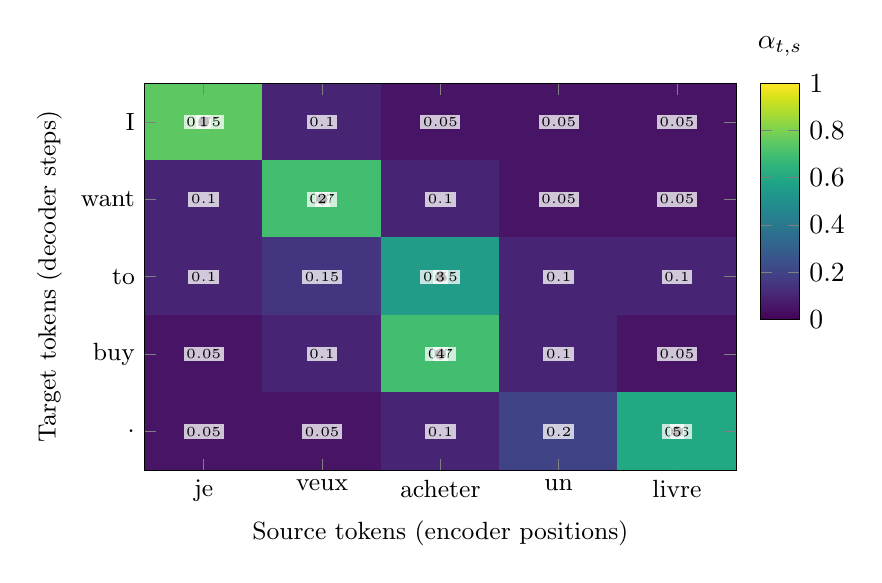
\begin{tikzpicture}
    \begin{axis}[
        width=0.75\linewidth,
        height=6.5cm,
        xlabel={Source tokens (encoder positions)},
        ylabel={Target tokens (decoder steps)},
        xtick={1,2,3,4,5},
        xticklabels={je,veux,acheter,un,livre},
        ytick={1,2,3,4,5},
        yticklabels={I,want,to,buy,.},
        y dir=reverse,
        colormap/viridis,
        colorbar,
        colorbar style={title={$\alpha_{t,s}$}, height=3.0cm},
        nodes near coords={\pgfmathprintnumber[fixed,precision=2]{\pgfplotspointmeta}},
        nodes near coords align={center},
        every node near coord/.append style={
            font=\tiny,
            fill=white,
            fill opacity=0.75,
            text opacity=1,
            inner sep=1pt
        },
        point meta min=0, point meta max=1,
        every axis/.append style={font=\small},
        enlargelimits=false,
        axis on top,
    ]
    % rows = target tokens, columns = source tokens
    \addplot[
        matrix plot*,
        mesh/cols=5,
        mesh/rows=5,
        point meta=explicit,
    ] table[row sep=\\, meta=z]{
    x y z\\
    % I
    1 1 0.75\\ 2 1 0.10\\ 3 1 0.05\\ 4 1 0.05\\ 5 1 0.05\\
    % want
    1 2 0.10\\ 2 2 0.70\\ 3 2 0.10\\ 4 2 0.05\\ 5 2 0.05\\
    % to
    1 3 0.10\\ 2 3 0.15\\ 3 3 0.55\\ 4 3 0.10\\ 5 3 0.10\\
    % buy
    1 4 0.05\\ 2 4 0.10\\ 3 4 0.70\\ 4 4 0.10\\ 5 4 0.05\\
    % .
    1 5 0.05\\ 2 5 0.05\\ 3 5 0.10\\ 4 5 0.20\\ 5 5 0.60\\
    };
    % highlight argmax per target token
    \addplot[only marks, mark=*, mark size=1.8pt] coordinates {
        (1,1)  % I -> je
        (2,2)  % want -> veux
        (3,3)  % to -> acheter
        (3,4)  % buy -> acheter
        (5,5)  % . -> livre
    };
    \end{axis}
    \end{tikzpicture}
    % Avoid inline math in captions; it wraps poorly in some EPUB renderers.
    \caption{Schematic: Attention heatmap for a translation model. Rows are target tokens (decoder steps) and columns are source tokens (encoder positions). Each cell is an attention weight; the dot in each row marks the source position receiving the most attention.}
    \label{fig:lec7-attention}
\end{figure}

\subsection{RNN Input-Output Configurations}

RNNs can be configured in several ways depending on the task:

\begin{itemize}
    \item \textbf{Many-to-Many (Equal Length):} Input and output sequences have the same length \( T \). For example, sequence labeling tasks.
    \item \textbf{Many-to-One:} Input is a sequence of length \( T \), output is a single prediction. Example: sentiment analysis where a sentence maps to a sentiment score.
    \item \textbf{Many-to-Many (Unequal Length):} Input and output sequences have different lengths. Example: machine translation where input and output sentences differ in length.
    \item \textbf{One-to-Many:} Single input produces a sequence output. Less common, but applicable in tasks like image captioning where one image input generates a sequence of words.
\end{itemize}

The main difference lies in how the loss is computed and how outputs are generated, but the underlying backpropagation principles remain consistent.

\subsection{Representing Words for RNN Inputs}

Natural language processing (NLP) requires converting words into numerical representations that RNNs can process. Since machines operate on numbers, words must be encoded appropriately.

\paragraph{Vocabulary Size and Word Representation}

Natural language has a large but finite vocabulary at any chosen granularity. Depending on whether you count words, inflections, or subword units, the effective inventory can range from tens of thousands (common token vocabularies) to far larger sets of distinct surface forms.

This finite vocabulary allows us to define a fixed-size dictionary \( V \) of words.

\paragraph{One-Hot Encoding}

A simple method to represent words is \emph{one-hot encoding}:
\begin{itemize}
    \item Assign each word in the vocabulary a unique index \( i \in \{1, \ldots, |V|\} \).
    \item Represent each word as a vector \( \mathbf{w} \in \mathbb{R}^{|V|} \) where all entries are zero except the \( i \)-th entry, which is 1.
\end{itemize}

For example, if \( |V| = 10,000 \), the word "house" might be represented as:
\[
\mathbf{w}_{\text{house}} = [0, 0, \ldots, 1, \ldots, 0],
\]
with the 1 in the position corresponding to "house".

This representation is sparse and high-dimensional. Conceptually the one-hot basis vectors correspond to the rows of the identity matrix \( I_{|V|} \), but in practice modern models replace that fixed basis with a \emph{learned} embedding table whose rows are trainable parameters. One convenient view is:
\[
\text{one-hot words} \;\leftrightarrow\; \text{rows of } I_{|V|},\qquad
\mathbf{E} \in \mathbb{R}^{|V|\times d}\ \text{trainable},\ \ \mathbf{e}_t = \mathbf{x}_t \mathbf{E},
\]
so a one-hot input \(\mathbf{x}_t\) simply selects the corresponding row of \(\mathbf{E}\) as its dense embedding \(\mathbf{e}_t\).

\paragraph{Limitations of One-Hot Encoding}

One-hot vectors do not capture semantic similarity between words (e.g., "king" and "queen" are orthogonal). Indeed, the cosine similarity between any two distinct one-hot vectors is exactly zero because their non-zero entries never overlap. They also lead to very high-dimensional inputs, which can be computationally costly to store and process.

To address these limitations we introduce distributed word representations (e.g., Word2Vec, GloVe, fastText) that map words to dense vectors where geometric relationships encode semantic similarity.

\subsection{Example: Sentiment Analysis with RNNs}

Consider the sentence:
\[
\text{"This place is great."}
\]

Each word is first converted into a numerical vector (e.g., one-hot encoded). The sequence of vectors is fed into the RNN, which processes them sequentially.

For a \emph{many-to-one} RNN (e.g., sentiment classification), we are interested in the hidden state after processing the entire sentence. This final hidden state summarizes the contextual information and can be fed into a classifier to predict the sentiment label.

\subsection{Limitations of One-Hot Encoding in Natural Language Processing}

Recall that one-hot encoding represents each word in the vocabulary as a unique vector with a single 1 and zeros elsewhere. While this approach guarantees uniqueness, it fails to capture any semantic or syntactic relationships between words.

\paragraph{Example:} Consider the sentences:
\begin{itemize}
    \item ``This place is great.''
    \item ``This place is awesome.''
    \item ``This place is good.''
\end{itemize}
Using one-hot encoding, the words \textit{great}, \textit{awesome}, and \textit{good} are represented as orthogonal vectors. Thus, a model trained to associate ``great'' with a five-star rating may not generalize to ``awesome'' or ``good,'' despite their similar meanings.

\paragraph{Document similarity:} Suppose we have two documents:
\begin{align*}
    D_1 &: \text{``I enjoyed talking to the monarchs.''} \\
    D_2 &: \text{``I loved conversing with the Royals.''}
\end{align*}
Semantically, these sentences convey the same meaning. However, one-hot encoding treats \textit{monarchs} and \textit{Royals} as distinct tokens, as well as \textit{talking} and \textit{conversing}. Consequently, simple word-count based similarity metrics (e.g., cosine similarity on bag-of-words vectors) would yield a low similarity score, failing to capture the semantic equivalence.

\paragraph{Summary:} One-hot encoding:
\begin{itemize}
    \item Ignores semantic similarity between words.
    \item Treats synonyms and related words as completely unrelated.
    \item Does not capture contextual or syntactic information.
\end{itemize}

This motivates the need for richer \textbf{feature representations} of words that encode their meanings and relationships.

\subsection{Feature-Based Word Representations}

To encode the meaning of words, we can represent each word as a vector of \emph{features} that capture semantic properties. These features can be handcrafted or learned, and aim to reflect qualities such as sentiment, category, or other linguistic attributes.

\paragraph{Example:} Consider the following words:
\[
\text{man, woman, king, queen, orange, apple, monarch, royal}
\]
We can define features such as:
\begin{itemize}
    \item \textbf{Gender}: male, female, neutral
    \item \textbf{Royalty status}: commoner, royalty
    \item \textbf{Age}: adult, child
    \item \textbf{Category}: animal, fruit, person, abstract
    \item \textbf{Edibility}: edible, inedible
    \item \textbf{Sweetness}: sweet, not sweet
\end{itemize}

Assigning numerical values to these features for each word yields a vector representation that encodes semantic information. For example:

\begin{center}
\small
\begin{tabular}{l|cccccccc}
\textbf{Word} & Gender & Royalty & Age & Person & Fruit & Title & Abstract & Sweet \\
\hline
man & 1 & 0 & 1 & 1 & 0 & 0 & 0 & 0 \\
woman & 0 & 0 & 1 & 1 & 0 & 0 & 0 & 0 \\
king & 1 & 1 & 1 & 1 & 0 & 1 & 0 & 0 \\
queen & 0 & 1 & 1 & 1 & 0 & 1 & 0 & 0 \\
orange & 0 & 0 & 0 & 0 & 1 & 0 & 0 & 1 \\
apple & 0 & 0 & 0 & 0 & 1 & 0 & 0 & 1 \\
monarch & 0.5 & 1 & 0.5 & 1 & 0 & 1 & 0 & 0 \\
royal & 0 & 1 & 0.5 & 0 & 0 & 1 & 1 & 0 \\
\end{tabular}
\end{center}

\paragraph{Notes:}
\begin{itemize}
    \item The values can be binary or continuous, reflecting degrees or uncertainty (e.g., ``monarch'' receives a gender value of 0.5 to indicate that the term is used for multiple genders).
    \item High-level categories are often represented with several binary indicators (person, fruit, title, abstract) rather than a single categorical feature.
    \item Some features may be language- or culture-specific, and this approach requires domain knowledge and manual feature engineering.
\end{itemize}

\paragraph{Advantages:}
\begin{itemize}
    \item Captures semantic similarity: words with similar features have similar representations.
    \item Enables reasoning about relationships (e.g., gender, royalty).
    \item Provides interpretable dimensions.
\end{itemize}

\paragraph{Limitations:}
\begin{itemize}
    \item Requires extensive manual effort to define and annotate features.
    \item May not scale well to large vocabularies or complex semantics.
    \item Difficult to capture contextual nuances and polysemy.
\end{itemize}

\subsection{Towards Distributed Word Representations}

The feature-based approach motivates the idea of \textbf{distributed representations}, where each word is represented as a dense vector in a continuous space. These vectors encode semantic and syntactic properties implicitly, often learned from large corpora.

\paragraph{Key idea:} Instead of one-hot vectors, represent each word \( w \) as a vector \(\mathbf{v}_w \in \mathbb{R}^d\), where \(d \ll |V|\) (vocabulary size), such that:
\[
\text{similarity}(\mathbf{v}_w, \mathbf{v}_{w'}) \approx \text{semantic similarity}(w, w')
\]

\paragraph{Methods to obtain distributed representations}
Several approaches learn such embeddings automatically from corpora, including neural language models (Word2Vec CBOW and Skip-gram), matrix factorization methods (GloVe), and contextual models (ELMo, BERT). These methods leverage co-occurrence statistics to place semantically similar words nearby in the embedding space.

\subsection{Semantic Relationships in Word Embeddings}

We continue our exploration of word embeddings by examining how semantic relationships between words can be captured in vector space. The key insight, as demonstrated by \citet{Mikolov2013}, is that certain linguistic regularities and patterns manifest as linear relationships between word vectors.
\paragraph{Subword tokenization and OOV handling.} Modern NLP systems rarely operate on raw word types alone. To reduce vocabulary size and handle out-of-vocabulary (OOV) words, they tokenize text into \emph{subword units}. Byte Pair Encoding (BPE) and WordPiece learn a compact inventory of frequent character sequences; words are segmented into a small number of subwords that can be re-composed by the model. FastText instead augments word vectors with character \(n\)-gram embeddings, so the representation of an unseen word is the sum of its subword vectors. Subword methods improve data efficiency, model morphology, and eliminate true OOVs while keeping sequence lengths manageable.

\paragraph{Example: Gender and Royalty Analogies}

Consider the analogy involving gender and royalty:

\[
\text{king} - \text{man} + \text{woman} \approx \text{queen}.
\]

This relationship suggests that the vector difference between \textit{king} and \textit{man} encodes the concept of "royal masculinity," and adding the vector for \textit{woman} shifts this to "royal femininity," yielding a vector close to \textit{queen}.

More formally, if we denote the embedding of a word \( w \) as \(\mathbf{v}_w\), then the analogy can be expressed as:

\begin{equation}
\mathbf{v}_{\text{king}} - \mathbf{v}_{\text{man}} + \mathbf{v}_{\text{woman}} \approx \mathbf{v}_{\text{queen}}.
\label{eq:king-queen-analogy}
\end{equation}

This vector arithmetic captures semantic relationships and can be used to find words that best complete analogies by maximizing cosine similarity:

\[
\arg\max_{w} \cos\big(\mathbf{v}_w, \mathbf{v}_{\text{king}} - \mathbf{v}_{\text{man}} + \mathbf{v}_{\text{woman}}\big).
\]

Here \(\cos(\mathbf{a}, \mathbf{b}) = \frac{\mathbf{a}^\top \mathbf{b}}{\|\mathbf{a}\|\,\|\mathbf{b}\|}\) denotes cosine similarity between vectors \(\mathbf{a}\) and \(\mathbf{b}\).

\paragraph{Empirical Validation}

Mikolov et al. showed that these relationships hold not only for gender and royalty but also for other semantic categories such as family relations (e.g., \textit{uncle} to \textit{aunt}), geographical locations (e.g., \textit{Portugal} to \textit{Lisbon}), and cultural concepts. The distances between word vectors reflect meaningful semantic distances, such as:

\[
\|\mathbf{v}_{\text{man}} - \mathbf{v}_{\text{woman}}\|_2 \approx \|\mathbf{v}_{\text{king}} - \mathbf{v}_{\text{queen}}\|_2,
\]

and similarly for other pairs.

\paragraph{Geographical and Cultural Clustering}

Word embeddings also often (empirically) capture geographic and cultural proximity. For example, the embeddings for countries and their capitals frequently cluster together:

\[
\mathbf{v}_{\text{Portugal}} \approx \mathbf{v}_{\text{Lisbon}}, \quad \mathbf{v}_{\text{Spain}} \approx \mathbf{v}_{\text{Madrid}}, \quad \mathbf{v}_{\text{France}} \approx \mathbf{v}_{\text{Paris}},
\]

and countries that are geographically close tend to have embeddings closer in vector space (e.g., \textit{China} is closer to \textit{Russia} and \textit{Japan} than to \textit{Portugal}), although the strength of this effect depends on the corpus used for training. Throughout this chapter, statements such as $\mathbf{v}_{\text{Portugal}} \approx \mathbf{v}_{\text{Lisbon}}$ are shorthand for ``the cosine similarity between the vectors exceeds a data-dependent threshold (typically $>0.8$)'' or, equivalently, that the two vectors lie in each other's $k$-nearest-neighbor list under cosine distance. These relations are empirical regularities rather than hard equalities, and the precise neighborhood structure depends on the corpus, training objective, and dimensionality of the embedding space.
\Cref{fig:lec7-embedding-clusters} illustrates such neighborhoods after projecting embeddings to two principal components; the visual clusters make the relational analogies immediately apparent.
\begin{figure}[t]
    \centering
    \includegraphics[width=\textwidth]{lec14_embeddings_clusters}
    % Avoid inline math in captions; it wraps poorly in some EPUB renderers.
    \caption{Schematic: Toy 2D projection of word embeddings showing neighboring clusters (countries vs. capitals). Light hulls highlight clusters; arrows show that country-to-capital displacement vectors align, a visual check on analogy structure.}
    \label{fig:lec7-embedding-clusters}
\end{figure}

\subsection{Feature-Based Representation vs. One-Hot Encoding}

The success of word embeddings lies in their ability to represent words as dense vectors encoding multiple latent features, as opposed to sparse one-hot vectors.

\paragraph{One-Hot Encoding}

One-hot encoding represents each word as a vector with a single 1 and zeros elsewhere. This representation is:

\begin{itemize}
    \item \textbf{Sparse}: High-dimensional with mostly zeros (in the one-hot representation used here, the dimensionality equals the vocabulary size and only one entry is non-zero for each word).
    \item \textbf{Uninformative}: No notion of similarity between words.
\end{itemize}

\paragraph{Feature-Based Embeddings}

In contrast, word embeddings are dense vectors in \(\mathbb{R}^d\) (typically \(d=100\) to \(300\)) where each dimension can be interpreted as a latent feature capturing semantic or syntactic properties. These features emerge from the training process rather than being explicitly defined. The term ``feature-based embedding'' is non-standard in the literature; we use it here simply to stress that the coordinates behave like automatically discovered features. Most papers instead refer to these objects as \emph{dense distributed representations}, and we always mean that same concept.
Unlike the hand-crafted example below, the latent dimensions of distributed embeddings are not usually interpretable in isolation. They capture statistical regularities uncovered automatically during training. Interpretability can sometimes be probed post hoc (e.g., via probing classifiers or dimension alignment), but there is no guarantee that any single axis corresponds cleanly to a human-understandable attribute.

\paragraph{Context Window Convention}

When we refer to the ``context'' of a word \(w_t\) we mean the multiset of tokens that fall within a symmetric sliding window of radius \(c\) around position \(t\). Formally,
\[
    \mathcal{C}_t = \{\,w_{t-c},\ldots,w_{t-1},\; w_{t+1},\ldots,w_{t+c}\,\}.
\]
Directional variants sometimes use only the preceding words. The co-occurrence matrix in the next section corresponds to the special case \(c=1\), where we only count the following token. Making the window definition explicit removes ambiguity about which neighboring words contribute counts to \(C_{ij}\).

\subsection{Open Questions: Feature Discovery and Representation}

Two natural questions arise regarding the nature of these features:

\begin{enumerate}
    \item \textbf{Who decides the features?}
    Unlike manually engineered features, the features in word embeddings are \emph{discovered automatically} during training. There is no explicit human selection of features such as "gender" or "age." Instead, the training algorithm uncovers latent dimensions that best capture word co-occurrence statistics.

    \item \textbf{How are the feature values determined?}
The feature values (vector components) are learned by optimizing an objective function that encourages words appearing in similar contexts to have similar embeddings. This is typically done via self-supervised learning on large corpora. In a self-supervised setting the model creates its own supervision signal (future tokens, masked tokens, or neighboring sentences), so that no external labels are required.
\end{enumerate}

\paragraph{Self-supervised learning of embeddings}

Although this learning is sometimes described informally as ``unsupervised,'' it is more accurately \emph{self-supervised} because the training objective uses the structure of the data itself (e.g., predicting context words) to create targets. In self-supervised setups the model manufactures its own targets from the input (for example, masking a word and asking the network to predict it), eliminating the need for manually annotated labels.

\paragraph{Summary}

Thus, the embedding process can be viewed as a function:

\[
f: \text{Vocabulary} \to \mathbb{R}^d,
\]

where \(f\) is learned to encode semantic and syntactic properties implicitly, without explicit feature engineering. In matrix form we implement \(f\) by selecting the \emph{row} of the learned embedding matrix \(\mathbf{E}\) corresponding to the word of interest (row\hyp{}embedding convention).

In practice we optimize objectives such as the continuous bag-of-words (CBOW) likelihood (predicts a center word from its surrounding context) and the skip-gram with negative sampling (SGNS) loss (predicts context words given a center word). These training regimes are typically optimized with SGD variants (SGD, Adam) on large corpora; \Cref{chap:nlp} spells out the CBOW/skip-gram objectives in detail.

% References:
% \begin{thebibliography}{9}
% \bibitem{mikolov2013distributed}
% Tomas Mik

\noindent\textbf{Forward pointer.} We cover Word2Vec/CBOW, skip-gram, and GloVe in \Cref{chap:nlp}; keep the self-supervised framing in mind as we shift from RNNs to dedicated embedding objectives.

\subsection{Wrapping Up the Derivations}

In this chapter, we have explored the foundational concepts behind modeling sequences in natural language processing (NLP) using recurrent neural networks (RNNs). We began by considering the problem of predicting the probability of a word given its preceding context, which is central to language modeling.

Recall that the goal is to estimate the conditional probability of a word \( w_t \) given the sequence of previous words \( w_1, w_2, \ldots, w_{t-1} \):
\begin{equation}
    P(w_t \mid w_1, w_2, \ldots, w_{t-1}).
\end{equation}

This probability can be modeled using an RNN, which maintains a hidden state \( \mathbf{h}_t \) that summarizes the history up to time \( t \). A common indexing choice is: consume the current token \(w_t\) (as an embedding \(\mathbf{x}_t\)) and predict the \emph{next} token \(w_{t+1}\). This is equivalent to modeling \(P(w_t\mid w_{1:t-1})\) after a one-step shift.
\begin{align}
    \mathbf{h}_t &= f(\mathbf{h}_{t-1}, \mathbf{x}_t; \theta), \\
    P(w_{t+1} \mid w_1, \ldots, w_t) &= g(\mathbf{h}_t; \theta), \label{eq:rnn_output_prob}
\end{align}
where \( \mathbf{x}_t \) is the input representation (e.g., word embedding) of the word \( w_t \), \( f \) is the recurrent update function parameterized by \(\theta\), and \( g \) maps the hidden state to a probability distribution over the vocabulary. Because the hidden state is computed recursively, \(\mathbf{h}_t\) already aggregates information about the entire prefix \((w_1,\ldots,w_t)\); predicting \(w_{t+1}\) from \(\mathbf{h}_t\) therefore reflects the Markovian summary that RNNs maintain. Explicitly, repeatedly substituting \Cref{eq:rnn_hidden_state} reveals that \(\mathbf{h}_t=f(f(\cdots f(\mathbf{h}_0,\mathbf{x}_1),\ldots),\mathbf{x}_t)\), so no information is lost other than the compression inherent to the finite-dimensional state vector.

\paragraph{Training Objective}

The network is trained to maximize the likelihood of the observed sequences in a large corpus of text. Given a training sequence \( (w_1, w_2, \ldots, w_T) \), the log-likelihood is:
\begin{equation}
    \mathcal{L}(\theta) = \sum_{t=1}^{T-1} \log P(w_{t+1} \mid w_1, \ldots, w_t; \theta).
\end{equation}

This objective encourages the model to assign high probability to the actual next word in the sequence, effectively learning the statistical structure of the language without explicit labeling of word relationships.

\paragraph{Self-supervised nature of language modeling}

A key insight is that no explicit labeling is required to train such models. The natural co-occurrence statistics of words in large corpora serve as implicit supervision. For example, the model learns that the word "juice" often follows "apple" because this pattern frequently appears in the training data. This is the essence of \emph{self-supervised} learning in NLP, where the prediction targets are created directly from the input sequence.

\paragraph{Feature Representations}

The input to the RNN is typically a dense vector representation of words, known as \emph{word embeddings}. These embeddings capture semantic and syntactic properties of words and are learned jointly with the model parameters. The embedding matrix \( \mathbf{E} \in \mathbb{R}^{V \times d} \), where \( V \) is the vocabulary size and \( d \) is the embedding dimension, maps each word index to a vector. We denote by \(\mathbf{e}_{w_t}\in\{0,1\}^{1\times V}\) the one-hot row indicator of word \(w_t\). The embedding lookup can then be written compactly as
\begin{equation}
    \mathbf{x}_t = \mathbf{e}_{w_t}\mathbf{E},
\end{equation}
so \(\mathbf{E}[w_t]\) simply selects the row of \(\mathbf{E}\) associated with \(w_t\). The boldface \(\mathbf{E}[\,\cdot\,]\) notation is intentional: it denotes array indexing into the learnable embedding matrix rather than an expectation operator \( \mathbb{E}[\cdot] \). Whenever expectations appear later in the book we write them explicitly as \( \mathbb{E}[\cdot] \) to avoid overload.

\paragraph{Summary of the Modeling Pipeline}

\begin{enumerate}
    \item Collect a large corpus of text data.
    \item Tokenize the text into sequences of words.
    \item Represent words as embeddings (initialized from a lookup table that is \emph{learned jointly} with the network parameters).
    \item Use an RNN to process sequences and produce hidden states.
    \item Predict the next word probability distribution from the hidden state.
    \item Train the model by maximizing the likelihood of the observed sequences.
\end{enumerate}

\begin{tcolorbox}[summarybox,title={LSTM and GRU equations (compact)}]
\textbf{LSTM} (single layer):
\[
\begin{aligned}
    \mathbf{i}_t &= \sigma(\mathbf{x}_t\mathbf{W}_i+\mathbf{h}_{t-1}\mathbf{U}_i+\mathbf{b}_i), &
    \mathbf{f}_t &= \sigma(\mathbf{x}_t\mathbf{W}_f+\mathbf{h}_{t-1}\mathbf{U}_f+\mathbf{b}_f), \\
    \tilde{\mathbf{c}}_t &= \tanh(\mathbf{x}_t\mathbf{W}_c+\mathbf{h}_{t-1}\mathbf{U}_c+\mathbf{b}_c), &
    \mathbf{o}_t &= \sigma(\mathbf{x}_t\mathbf{W}_o+\mathbf{h}_{t-1}\mathbf{U}_o+\mathbf{b}_o), \\
    \mathbf{c}_t &= \mathbf{f}_t\odot \mathbf{c}_{t-1} + \mathbf{i}_t\odot \tilde{\mathbf{c}}_t, &
    \mathbf{h}_t &= \mathbf{o}_t\odot \tanh(\mathbf{c}_t).
\end{aligned}
\]
\textbf{GRU}:
\[
\begin{aligned}
    \mathbf{z}_t &= \sigma(\mathbf{x}_t\mathbf{W}_z+\mathbf{h}_{t-1}\mathbf{U}_z+\mathbf{b}_z), &
    \mathbf{r}_t &= \sigma(\mathbf{x}_t\mathbf{W}_r+\mathbf{h}_{t-1}\mathbf{U}_r+\mathbf{b}_r), \\
    \tilde{\mathbf{h}}_t &= \tanh(\mathbf{x}_t\mathbf{W}_h+(\mathbf{r}_t\odot\mathbf{h}_{t-1})\mathbf{U}_h+\mathbf{b}_h), &
    \mathbf{h}_t &= (1-\mathbf{z}_t)\odot \mathbf{h}_{t-1} + \mathbf{z}_t\odot \tilde{\mathbf{h}}_t.
\end{aligned}
\]
All gates are elementwise; $\sigma$ denotes the logistic sigmoid and $\odot$ the Hadamard product.

\paragraph{Notation note.} In the sequence\hyp{}model chapters, $\sigma(\cdot)$ always denotes the logistic sigmoid gate nonlinearity; when $\sigma$ is used without an argument (e.g., in earlier chapters for noise scales $\sigma^2$) it refers to a standard deviation. Context distinguishes these roles.
\end{tcolorbox}

\begin{tcolorbox}[summarybox,title={Key takeaways}]
\begin{itemize}
    \item Language modeling is trained with self-supervision by maximizing next-token likelihood.
    \item Embeddings provide dense, learned word features; RNN hidden states encode context.
    \item Stability tools (clipping, gating, attention) enable long-range dependency modeling.
\end{itemize}
\end{tcolorbox}

\begin{tcolorbox}[summarybox,title={Exercises and lab ideas}]
\begin{itemize}
    \item Train a many-to-one sentiment classifier; plot gradient norms with and without clipping.
    \item Train a small LSTM language model; compare perplexity with/without weight tying and scheduled sampling.
    \item Empirically sweep \(\|\mathbf{W}_{hh}\|\) (spectral scaling) and reproduce vanishing/exploding behavior.
    \item Implement the masked, truncated-BPTT loop above and verify that pads do not affect the loss.
\end{itemize}
\end{tcolorbox}

\medskip
\paragraph{Where we head next.} RNNs excel at streaming and moderate-context tasks but struggle with very long dependencies and parallel hardware utilization. \Cref{chap:transformers} introduces attention/Transformers to address these limits; \Cref{chap:nlp} revisits embeddings, perplexity, and weight tying \citep{Press2016} that pair naturally with RNN language models.

\paragraph{References.} Full citations for works mentioned in this chapter appear in the book-wide bibliography.
\nocite{JurafskyMartin2023,Goodfellow2016,Mikolov2010,LevyGoldberg2014}
